\documentclass[a0paper,final,landscape]{baposter}
\usepackage{lmodern}
\usepackage[utf8]{inputenc} 
\usepackage{relsize}
\usepackage{varwidth}
\usepackage{caption}
\usepackage{varwidth}
\usepackage{caption}
\usepackage{graphicx}
\usepackage{svg}
\usepackage{pst-node} 
\usepackage[utf8]{inputenc}
\usepackage{pgfplots}
\usetikzlibrary{matrix}
\usepgfplotslibrary{groupplots}
\pgfplotsset{compat=newest}
\usepackage{fontawesome}


\usepackage{pgfbaselayers}
\pgfdeclarelayer{background}
\pgfdeclarelayer{foreground}
\pgfsetlayers{background,main,foreground}

\usepackage{enumitem}
\usepackage{amsmath,amsfonts,amsthm,amssymb}
\usepackage{mathtools}
\usepackage{siunitx}
\usepackage{fontawesome}
\usepackage{lmodern}
%\usepackage{chemmacros}
%\usepackage{authblk}

% \newcommand{\captionfont}{\footnotesize}

\selectcolormodel{cmyk}
\graphicspath{{images/}}

\captionsetup[figure]{font={sf, small}}

%%%%%%%%%%%%%%%%%%%%%%%%%%%%%%%%%%%%%%%%%%%%%%%%%%%%%%%%%%%%%%%%%%%%%%%%%%%%%%%%
%%%% Some math symbols used in the text
%%%%%%%%%%%%%%%%%%%%%%%%%%%%%%%%%%%%%%%%%%%%%%%%%%%%%%%%%%%%%%%%%%%%%%%%%%%%%%%%
% Format
\newcommand\myfrac[2]{\genfrac{}{}{0pt}{#1}{#2}}
\newcommand{\Matrix}[1]{\begin{bmatrix} #1 \end{bmatrix}}
\newcommand{\Vector}[1]{\Matrix{#1}}
\newcommand*{\SET}[1]  {\ensuremath{\mathcal{#1}}}
\newcommand*{\MAT}[1]  {\ensuremath{\mathbf{#1}}}
\newcommand*{\VEC}[1]  {\ensuremath{\bm{#1}}}
\newcommand*{\CONST}[1]{\ensuremath{\mathit{#1}}}
\newcommand*{\norm}[1]{\mathopen\| #1 \mathclose\|}% use instead of $\|x\|$
\newcommand*{\abs}[1]{\mathopen| #1 \mathclose|}% use instead of $\|x\|$
\newcommand*{\absLR}[1]{\left| #1 \right|}% use instead of $\|x\|$

\usepackage{xspace}
\newcommand{\id}{\ensuremath{1 \! \! \mathbb{I}}}
\newcommand{\eg}{e.g.,\xspace}
\newcommand{\Eg}{E.g.,\xspace}
\newcommand{\ie}{i.e.,\xspace}
\newcommand{\wo}{wo.\xspace}
\newcommand{\etal}{\emph{et al.}\xspace}
\newcommand{\cf}{cf.\xspace}
\newcommand{\invitro}{in vitro\xspace}
\newcommand{\Invitro}{In vitro\xspace}
\newcommand{\MP}{M$\Phi$\xspace}
\newcommand{\dd}{\ensuremath{\, \mathrm{d}}}

\newcommand{\lb}{\ensuremath{\left(}}
\newcommand{\rb}{\ensuremath{\right)}}
\newcommand{\lsb}{\ensuremath{\left[\,}}
\newcommand{\rsb}{\ensuremath{\, \right]}}
\newcommand{\BigOh}[1]{\ensuremath{\mathcal{O}(#1)}}

\newcommand{\nonlocalgrad}[1]{\ensuremath{\,\overset{\circ}{\nabla}_{#1}\;}}
\newcommand{\ngrad}{\ensuremath{\nonlocalgrad{R}}}
\def\norm#1{\mathopen\| #1 \mathclose\|}% use instead of $\|x\|$
\newcommand{\normLR}[1]{\left\| #1 \right\|}% use instead of $\|x\|$
\newcommand{\kraft}{\ensuremath{\boldsymbol{p}}}
\newcommand{\supp}{\mathop{\mathrm{supp}}}

\newcommand{\cinterval}[1]{\ensuremath{\left[#1\right]}}
\newcommand{\sgn}{\operatorname{sgn}}
\newcommand{\defeq}{\mathrel{\mathop:}=}
\newcommand{\eqdef}{\mathrel{\mathop=}:}

\theoremstyle{plain}
\newtheorem{lemma}{Lemma}

\theoremstyle{definition}
\newtheorem{definition}{Definition}

\definecolor{MidnightBlue}{cmyk}{0.78,0.78,0,0.56}
\definecolor{DarkViolet}{cmyk}{0.30,1.00,0.00,0.17} 
\definecolor{PiggyPink}{cmyk}{0, 0.7808, 0.4429, 0.1412}

%%%%%%%%%%%%%%%%%%%%%%%%%%%%%%%%%%%%%%%%%%%%%%%%%%%%%%%%%%%%%%%%%%%%%%%%%%%%%%%%
% Multicol Settings
%%%%%%%%%%%%%%%%%%%%%%%%%%%%%%%%%%%%%%%%%%%%%%%%%%%%%%%%%%%%%%%%%%%%%%%%%%%%%%%%
\setlength{\columnsep}{0.7em}
\setlength{\columnseprule}{0mm}

%%%%%%%%%%%%%%%%%%%%%%%%%%%%%%%%%%%%%%%%%%%%%%%%%%%%%%%%%%%%%%%%%%%%%%%%%%%%%%%%
% Save space in lists. Use this after the opening of the list
%%%%%%%%%%%%%%%%%%%%%%%%%%%%%%%%%%%%%%%%%%%%%%%%%%%%%%%%%%%%%%%%%%%%%%%%%%%%%%%%
\newcommand{\compresslist}{%
\setlength{\itemsep}{1pt}%
\setlength{\parskip}{0pt}%
\setlength{\parsep}{0pt}%
}

%%%%%%%%%%%%%%%%%%%%%%%%%%%%%%%%%%%%%%%%%%%%%%%%%%%%%%%%%%%%%%%%%%%%%%%%%%%%%%
%%% Begin of Document
%%%%%%%%%%%%%%%%%%%%%%%%%%%%%%%%%%%%%%%%%%%%%%%%%%%%%%%%%%%%%%%%%%%%%%%%%%%%%%
\newenvironment{flushenum}{%
 \begin{enumerate}[leftmargin=0.25cm,itemindent=.5cm,labelwidth=\itemindent,
         labelsep=0cm,align=left,itemsep=0em,parsep=0pt,topsep=0.1cm,label=\bfseries\arabic*.]
  \compresslist
  \setlength{\leftmargin}{0pt}
}{\end{enumerate}}

\newenvironment{flushitem}{%
\begin{itemize}[leftmargin=0.25cm,itemindent=.5cm,labelwidth=\itemindent,
labelsep=0cm,align=left,itemsep=0em,parsep=0pt]
  \compresslist
  \setlength{\leftmargin}{0pt}
}{\end{itemize}}

\def\twitter{{\small \FA \faTwitter}}
\def\home{{\small \FA \faHome}}
\def\homeLarge{{\huge \FA \faHome}}
\def\mail{{\small \FA \faEnvelopeAlt}}

\begin{document}

%%%%%%%%%%%%%%%%%%%%%%%%%%%%%%%%%%%%%%%%%%%%%%%%%%%%%%%%%%%%%%%%%%%%%%%%%%%%%%
%%% Here starts the poster
%%%---------------------------------------------------------------------------
%%% Format it to your taste with the options
%%%%%%%%%%%%%%%%%%%%%%%%%%%%%%%%%%%%%%%%%%%%%%%%%%%%%%%%%%%%%%%%%%%%%%%%%%%%%%
\typeout{Poster Starts}
% \background{
%   \begin{tikzpicture}[remember picture,overlay]%
%     \draw (current page.north west)+(-2em,-0em) node[anchor=north west] {\hspace{-2em}\includegraphics[height=1.1\textheight]{silhouettes_background}};
%   \end{tikzpicture}%
% }
%\definecolor{silver}{cmyk}{0,0,0,0.3}
% \definecolor{yellow}{cmyk}{0,0,0.9,0.0}
% \definecolor{reddishyellow}{cmyk}{0,0.22,1.0,0.0}
%\definecolor{black}{cmyk}{0,0,0.0,1.0}
% \definecolor{darkYellow}{cmyk}{0,0,1.0,0.5}
%\definecolor{darkSilver}{cmyk}{0,0,0,0.1}

\definecolor{UAgreen}{RGB}{0,124,65}
\definecolor{UAblack}{RGB}{0,0,0}
\definecolor{UAorange}{RGB}{255,160,35}
\definecolor{darkorange}{cmyk}{0.00,0.6,1.00,0.08}
\definecolor{lightgreen}{RGB}{210,255,210}
\definecolor{lightergreen}{RGB}{234,255,234}
\definecolor{lightestgreen}{cmyk}{0,0,0.05,0.0}

\begin{poster}{%
  % Show grid to help with alignment
  grid=false,
  columns=3,
  % Column spacing
  colspacing=1em,
  bgColorOne=white,
  % Background color for the gradient on the left side of the poster
  bgColorTwo=white,
  % Background color for the gradient on the right side of the right side
  borderColor=black, % Border color
  headerColorOne=MidnightBlue, % Background color for the header in the content
  % boxes l
  headerColorTwo=MidnightBlue, % Background color for the header in the content
  % boxes r
  headerFontColor=white, % Text color for the header text in the content
  % boxes
  % boxColorOne=lightestgreen, % Background color of the content boxes
  % boxColorTwo=lightestgreen,
  boxColorOne=white, % Background color of the content boxes
  boxColorTwo=white,
  % Format of textbox
  textborder=roundedleft,
  % Format of text header
  eyecatcher=true,
  headerborder=open,
  headerheight=0.12\textheight,
  headershape=roundedright,
  headershade=plain,
  headerfont=\large\bfseries\textsf, %Sans Serif
  boxshade=plain,
  background=shadeTB,
  linewidth=2.5pt
  }
  % Eye Catcher
  {%
  {\begin{minipage}{5em}
    \vspace{1em}
    
\includegraphics[height=8em]{./imagesnew/a-udem-logo2.png} 
  \hfill
  \end{minipage}
  }
  } % No eye catcher for this poster. If an eye catcher is present, the title
  % is centered between eye-catcher and logo.
  % Title
  {\sf\huge\bfseries\centering %Sans Serif
  %\bf% Serif
  % Evolving diverse genetic circuits by GFlowNet. 
  Evolving diverse gene networks
  }
  % Authors
  {\centering\sf %Sans Serif
  % Serif
  Qichen Huang,
  Nacer Eddine Boukacem,
  Paul François\hspace{3em}\\
  {\smaller
      % Client: Andrea Ku, MSc Candidate at UBC Department of Geography\\
      Supervised by Professors Paul François, Université de Montréal, Mila Quebec AI Institute\\
  }
  }

  %\tikzstyle{light shaded}=[top color=baposterBGtwo!30!white,bottom color=baposterBGone!30!white,shading=axis,shading angle=30]

  % Width of left inset image

%%%%%%%%%%%%%%%%%%%%%%%%%%%%%%%%%%%%%%%%%%%%%%%%%%%%%%%%%%%%%%%%%%%%%%%%%%%%%%
%%% Now define the boxes that make up the poster
%%%---------------------------------------------------------------------------
%%% Each box has a name and can be placed absolutely or relatively.
%%% The only inconvenience is that you can only specify a relative position
%%% towards an already declared box. So if you have a box attached to the
%%% bottom, one to the top and a third one which should be in between, you
%%% have to specify the top and bottom boxes before you specify the middle
%%% box.
%%%%%%%%%%%%%%%%%%%%%%%%%%%%%%%%%%%%%%%%%%%%%%%%%%%%%%%%%%%%%%%%%%%%%%%%%%%%%%
%
% A coloured circle useful as a bullet with an adjustably strong filling
\newcommand{\colouredcircle}[1]{%
  \tikz{\useasboundingbox (-0.2em,-0.32em) rectangle(0.2em,0.32em);
\draw[draw=black,fill=baposterBGone!80!black!#1!white,line width=0.03em] (0,0)
circle(0.18em);}}

%%%%%%%%%%%%%%%%%%%%%%%%%%%%%%%%%%%%%%%%%%%%%%%%%%%%%%%%%%%%%%%%%%%%%%%%%%%%%%
\headerbox{Objectives}{name=introduction,column=0,row=0}{%
%%%%%%%%%%%%%%%%%%%%%%%%%%%%%%%%%%%%%%%%%%%%%%%%%%%%%%%%%%%%%%%%%%%%%%%%%%%%%%

{\fontfamily{lmss}\selectfont
We propose leveraging GFlowNet, a novel machine learning approach, to generate diverse and functional Gene Regulatory Networks (GRNs). Our aim is to efficiently explore the vast space of GRNs associated with given functions, gain insights into their evolutionary plasticity, and potentially uncover general network motifs with improved performance or robustness. We focus on classical examples like genetic oscillators before advancing to more complex functions such as developmental patterning and T cell recognition dynamics.
}

}

%\headerbox{Objective}{name=objective,column=0,below=introduction}{\bfseries
%%
%Derive model~\eqref{Eqn:ArmstrongModel} from an underlying stochastic random
%walk.
%%
%}


%%%%%%%%%%%%%%%%%%%%%%%%%%%%%%%%%%%%%%%%%%%%%%%%%%%%%%%%%%%%%%%%%%%%%%%%%%%%%%
\headerbox{Introduction}{name=master,column=0,below=introduction}{%
%%%%%%%%%%%%%%%%%%%%%%%%%%%%%%%%%%%%%%%%%%%%%%%%%%%%%%%%%%%%%%%%%%%%%%%%%%

{\bf{\textsf{Research Questions}}}
{\fontfamily{lmss}\selectfont
\begin{flushenum}
    \item What are some diverse motifs associated with specific functions? 
    \item What are some common core motifs during evolution?
    \item How do GRNs evolve over time from oscillators to somitogenesis? 
\end{flushenum}
} 

\vspace{0.8em}

{\bf{\textsf{C\&P Architectures in Evolution}}}
\vspace{-0.2em}
\begin{center}
    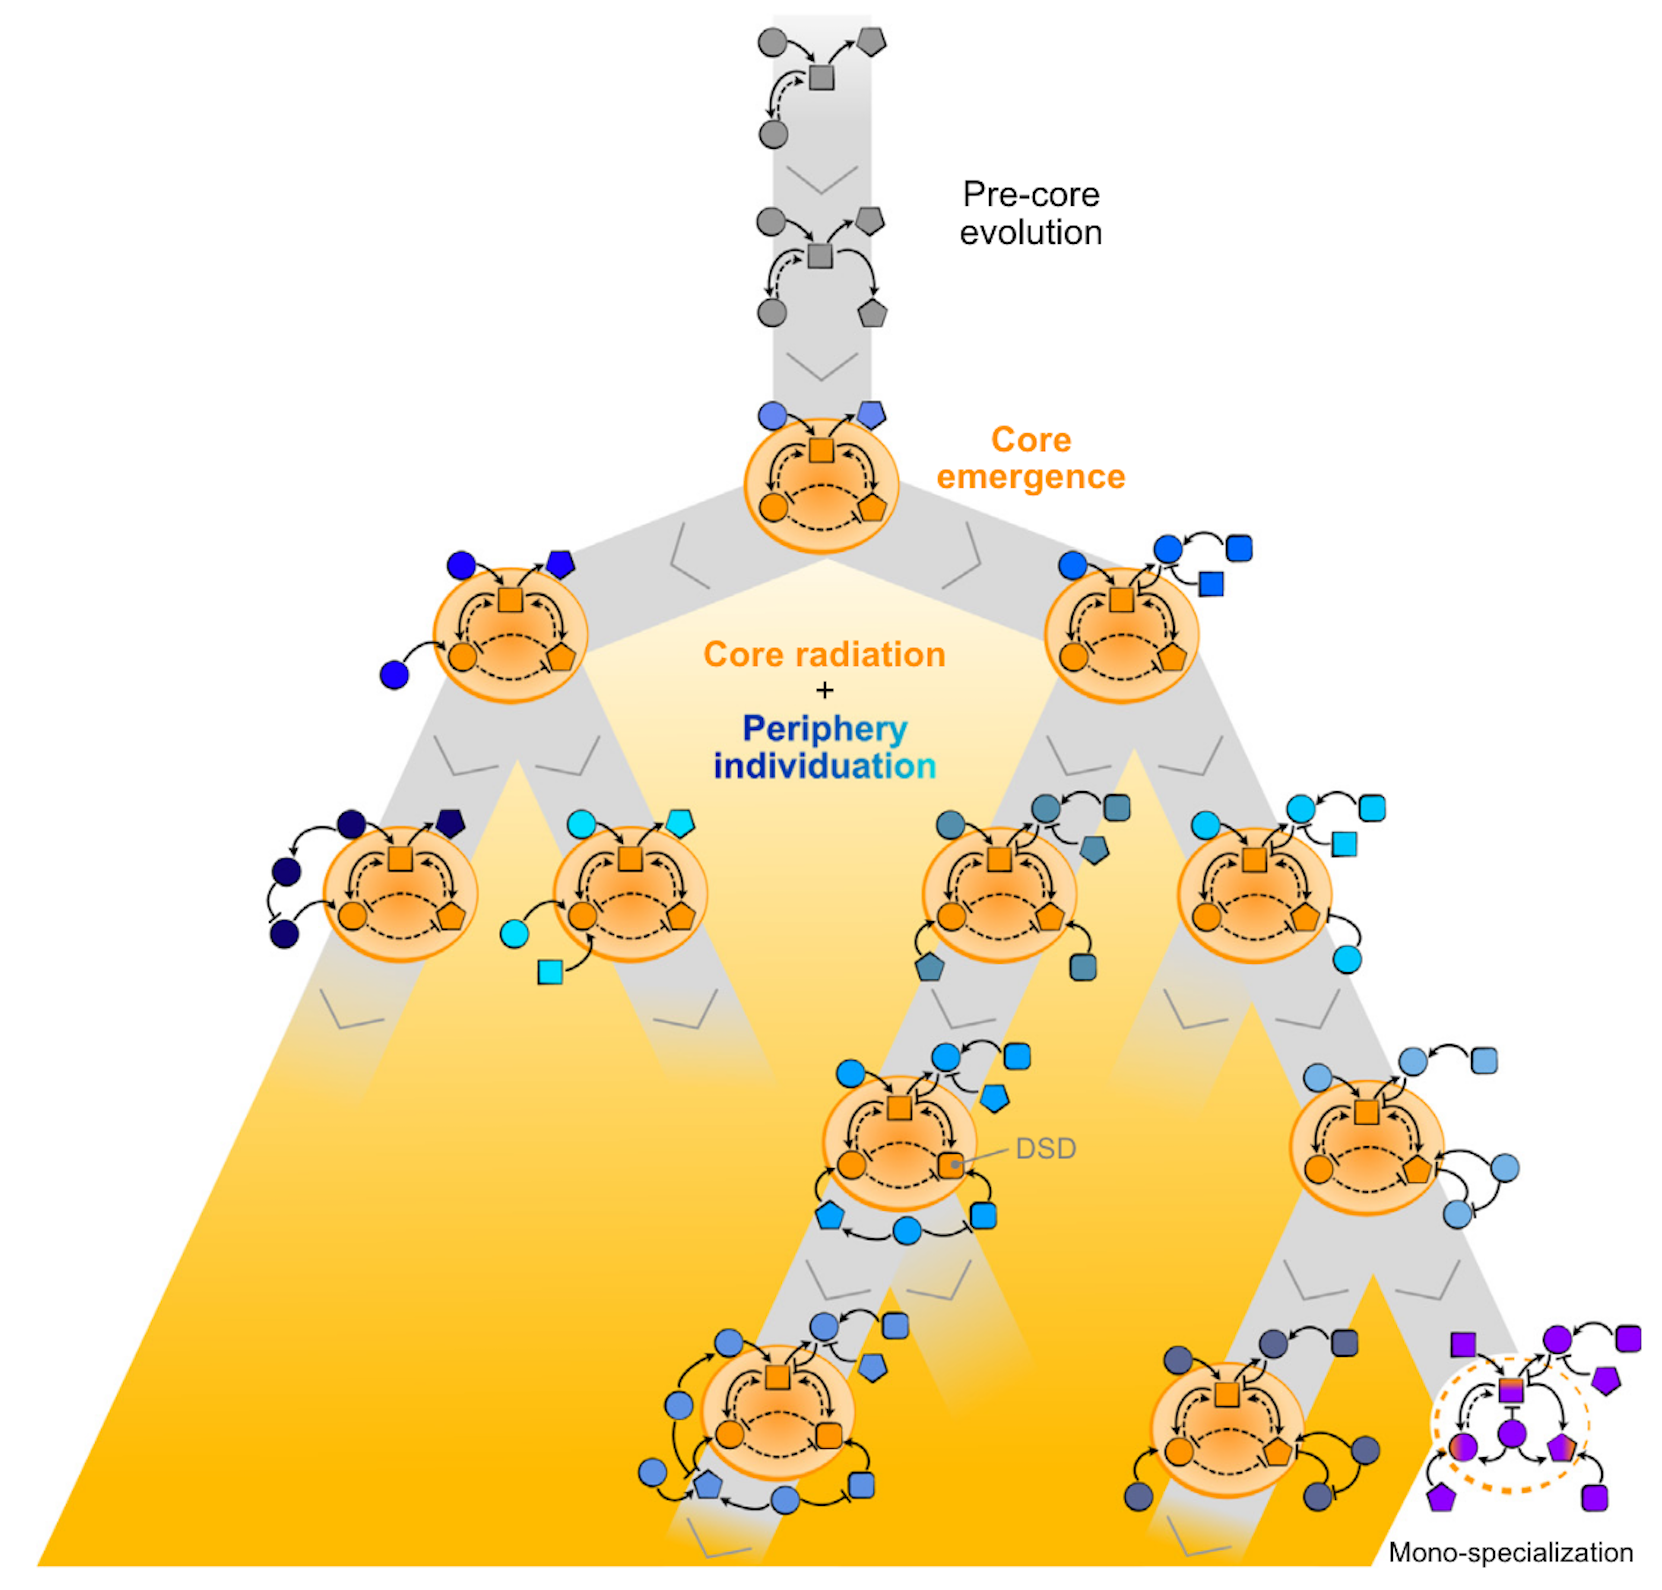
\includegraphics[width=0.4\textwidth]{./imagesnew/core-hypothese.png}
    \captionof{figure}{
    {\fontfamily{lmss}\selectfont
    The C\&P architectures in evolution, reused from (Gallo et al., 2024). Our model aligns with the \textit{core and periphery (C\&P) hypothesis}, providing insights into the evolutionary basis of GRNs.
    }
    }
\end{center}

\vspace{0.8em}

{\bf{\textsf{DAG Trajectories of GFlowNets}}}
\vspace{0.2em}
\begin{center}
    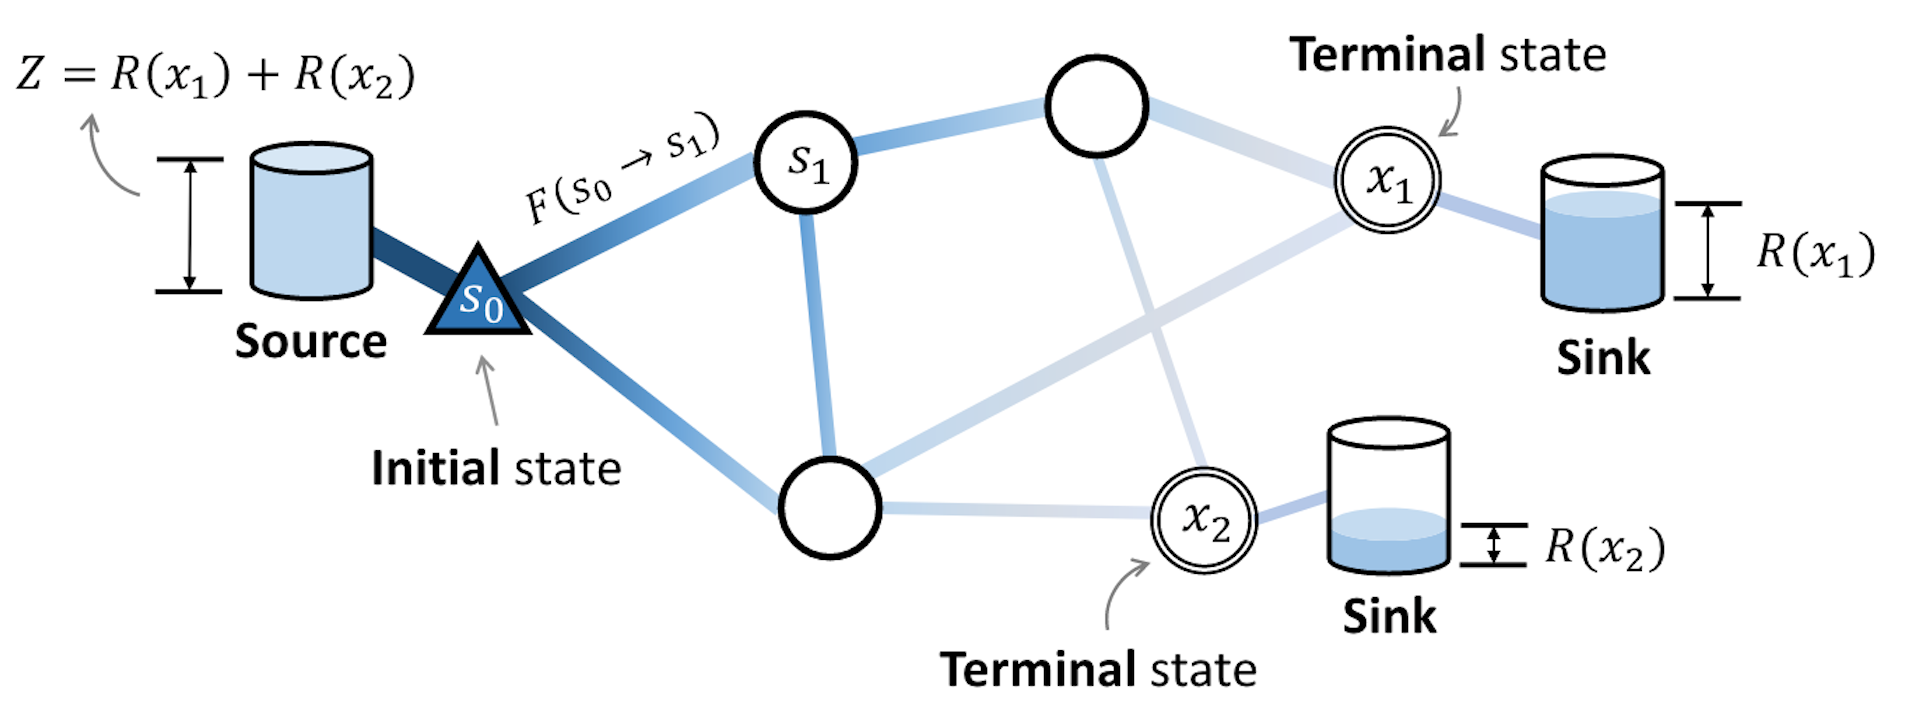
\includegraphics[width=0.9\textwidth]{./imagesnew/gfn-illustration.png}
    \captionof{figure}{
    {\fontfamily{lmss}\selectfont
    Illustration of generative flow network model, reused from (Kim et al., 2023). GFlowNet can efficiently explore the vast space of possible GRN configurations, allowing for more diverse candidate generation.
    }
    }
\end{center}


% {\bf{\textsf{Regionalization}}}
% {\fontfamily{lmss}\selectfont
% \vspace{-0.7em}
% \begin{flushitem}
%     \item Aim to cluster SEA into “similar” regions by fire patterns using Spatial 'K'luster Analysis by Tree Edge Removal (SKATER) algorithm.
% \end{flushitem}
% }


% {\bf{\textsf{Statistical Analysis}}}
% \vspace{-0.7em}
% {\fontfamily{lmss}\selectfont
% \begin{flushitem}
%     \item Analyze model performance and variable importance by Generalized Additive Models (GAM) and Random Forest Regression (RF).
% \end{flushitem}
% }

}

%%%%%%%%%%%%%%%%%%%%%%%%%%%%%%%%%%%%%%%%%%%%%%%%%%%%%%%%%%%%%%%%%%%%%%%%%%
\headerbox{Results on diverse oscillators}{name=rfr, column=1, row = 0}{
%%%%%%%%%%%%%%%%%%%%%%%%%%%%%%%%%%%%%%%%%%%%%%%%%%%%%%%%%%%%%%%%%%%%%%

{\bf{\textsf{Dynamical System Model}}}\\
\vspace{-1.7em}
\begin{center}
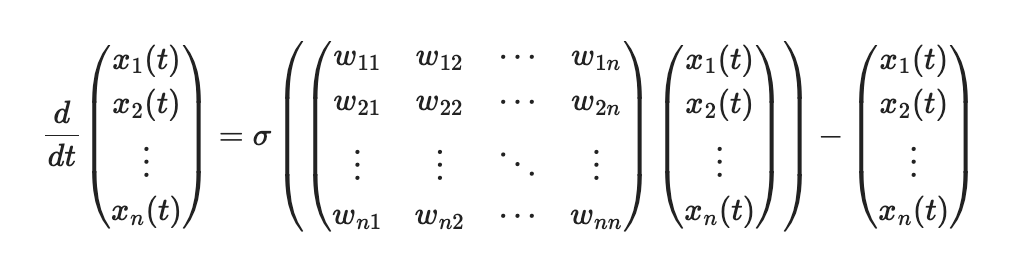
\includegraphics[width = 0.7\textwidth]{./imagesnew/dynamical-sys.png}
\vspace{-1.0em}
\captionof{figure}{
{\fontfamily{lmss}\selectfont
\textbf{Global Search GFN}: The state space $S$ is a finite set of states where each state represents an adjacency matrix. The action space $A = \{\pm1, \pm2, \pm4, \text{stop}\}$ where each action corresponds to enhancing or repressing the gene expression, or terminating the MDP. The reward function at the terminal state $R(x)$ is defined by the number of peaks produced by the oscillator. \textbf{Local Search GFN}: We initiate another GFN at high reward state with $A = \{\pm0.2, \pm0.5, \pm1, \text{stop}\}$ to perform local reward searching. 
}
}
\end{center}

{\bf{\textsf{3 Node Oscillator}}}\\
\vspace{-1.7em}
\begin{center}
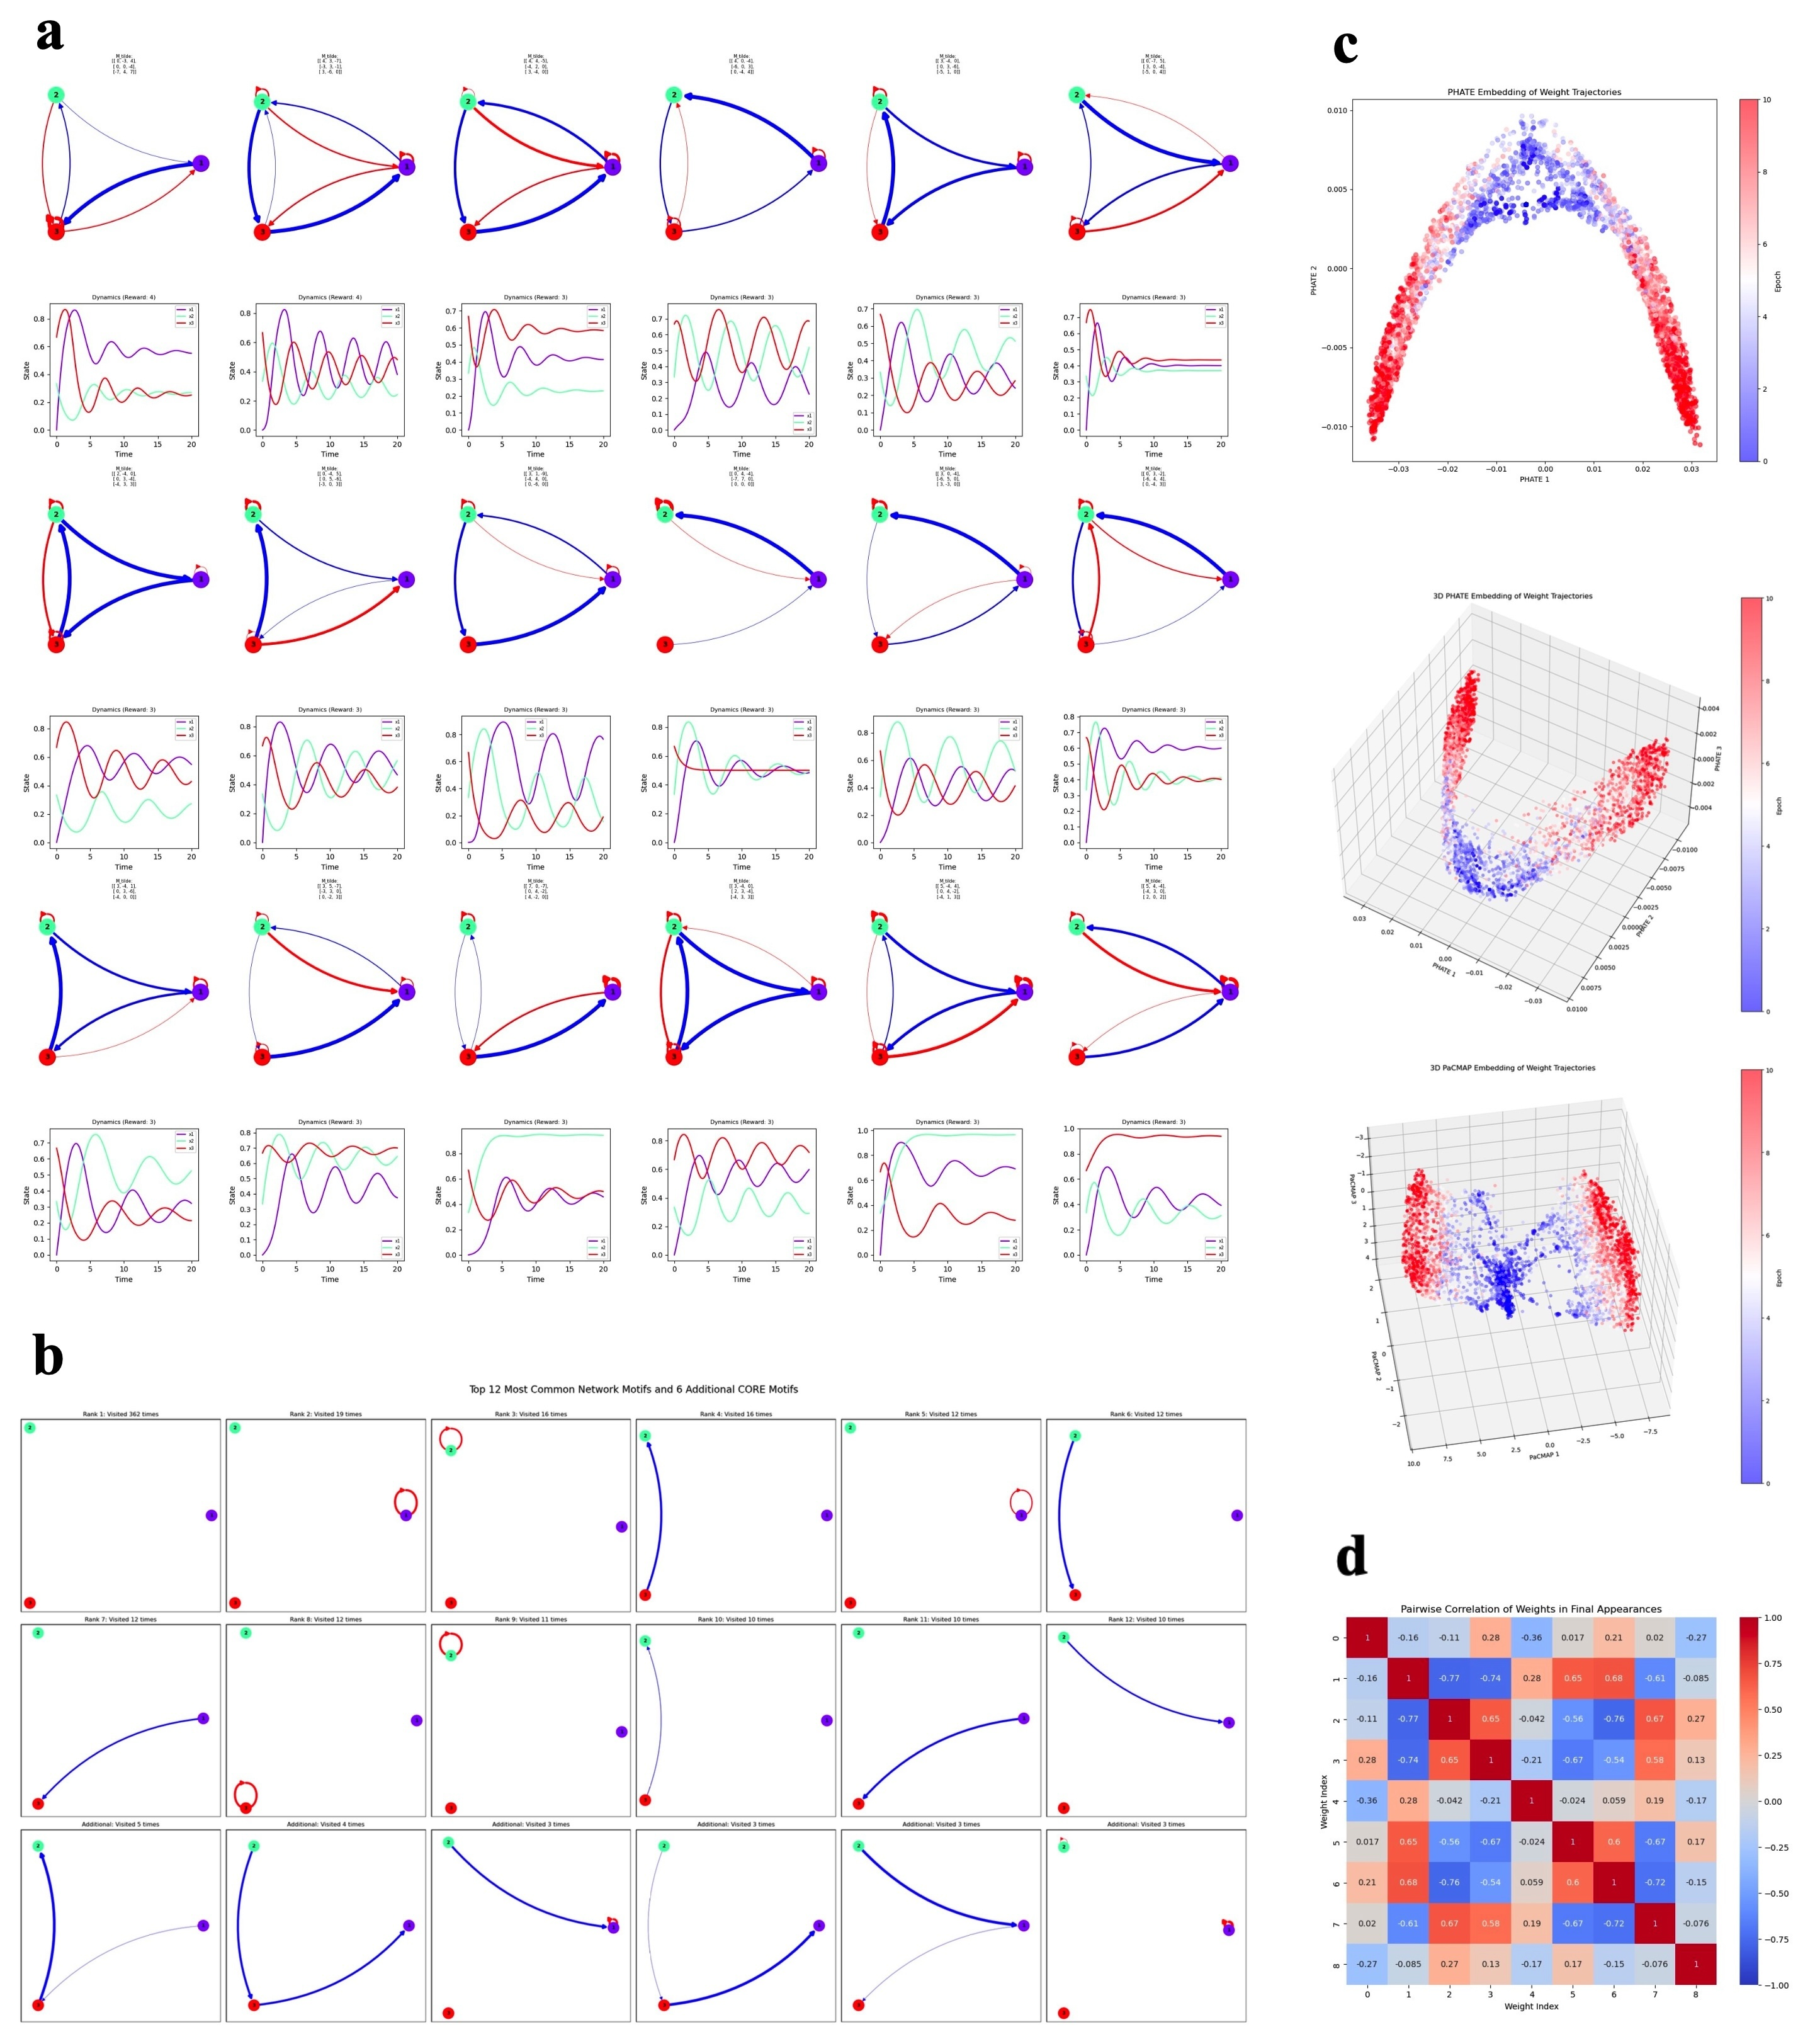
\includegraphics[width = 0.98\textwidth]{./imagesnew/3-node-combined.jpg}
\vspace{-0.6em}
\captionof{figure}{
{\fontfamily{lmss}\selectfont
Diverse motifs with gene 1 exhibiting 4 oscillations: (a) Various motifs achieving the desired oscillation. (b) Common Network Motifs representing intersections of all trajectories. (c) PHATE and PaCMAP visualization of all trajectories. (d) Pairwise correlation of weights in the terminal state. 
}
}
\end{center}

}

%%%%%%%%%%%%%%%%%%%%%%%%%%%%%%%%%%%%%%%%%%%%%%%%%%%%%%%%%%%%%%%%%%%%%%%%%%
\headerbox{Results on diverse segmentation}{name=performance, column=2, row=0}{
%%%%%%%%%%%%%%%%%%%%%%%%%%%%%%%%%%%%%%%%%%%%%%%%%%%%%%%%%%%%%%%%%%%%%%

{\bf{\textsf{Segmentation Networks}}}\\
\vspace{-0.7em}
\begin{center}
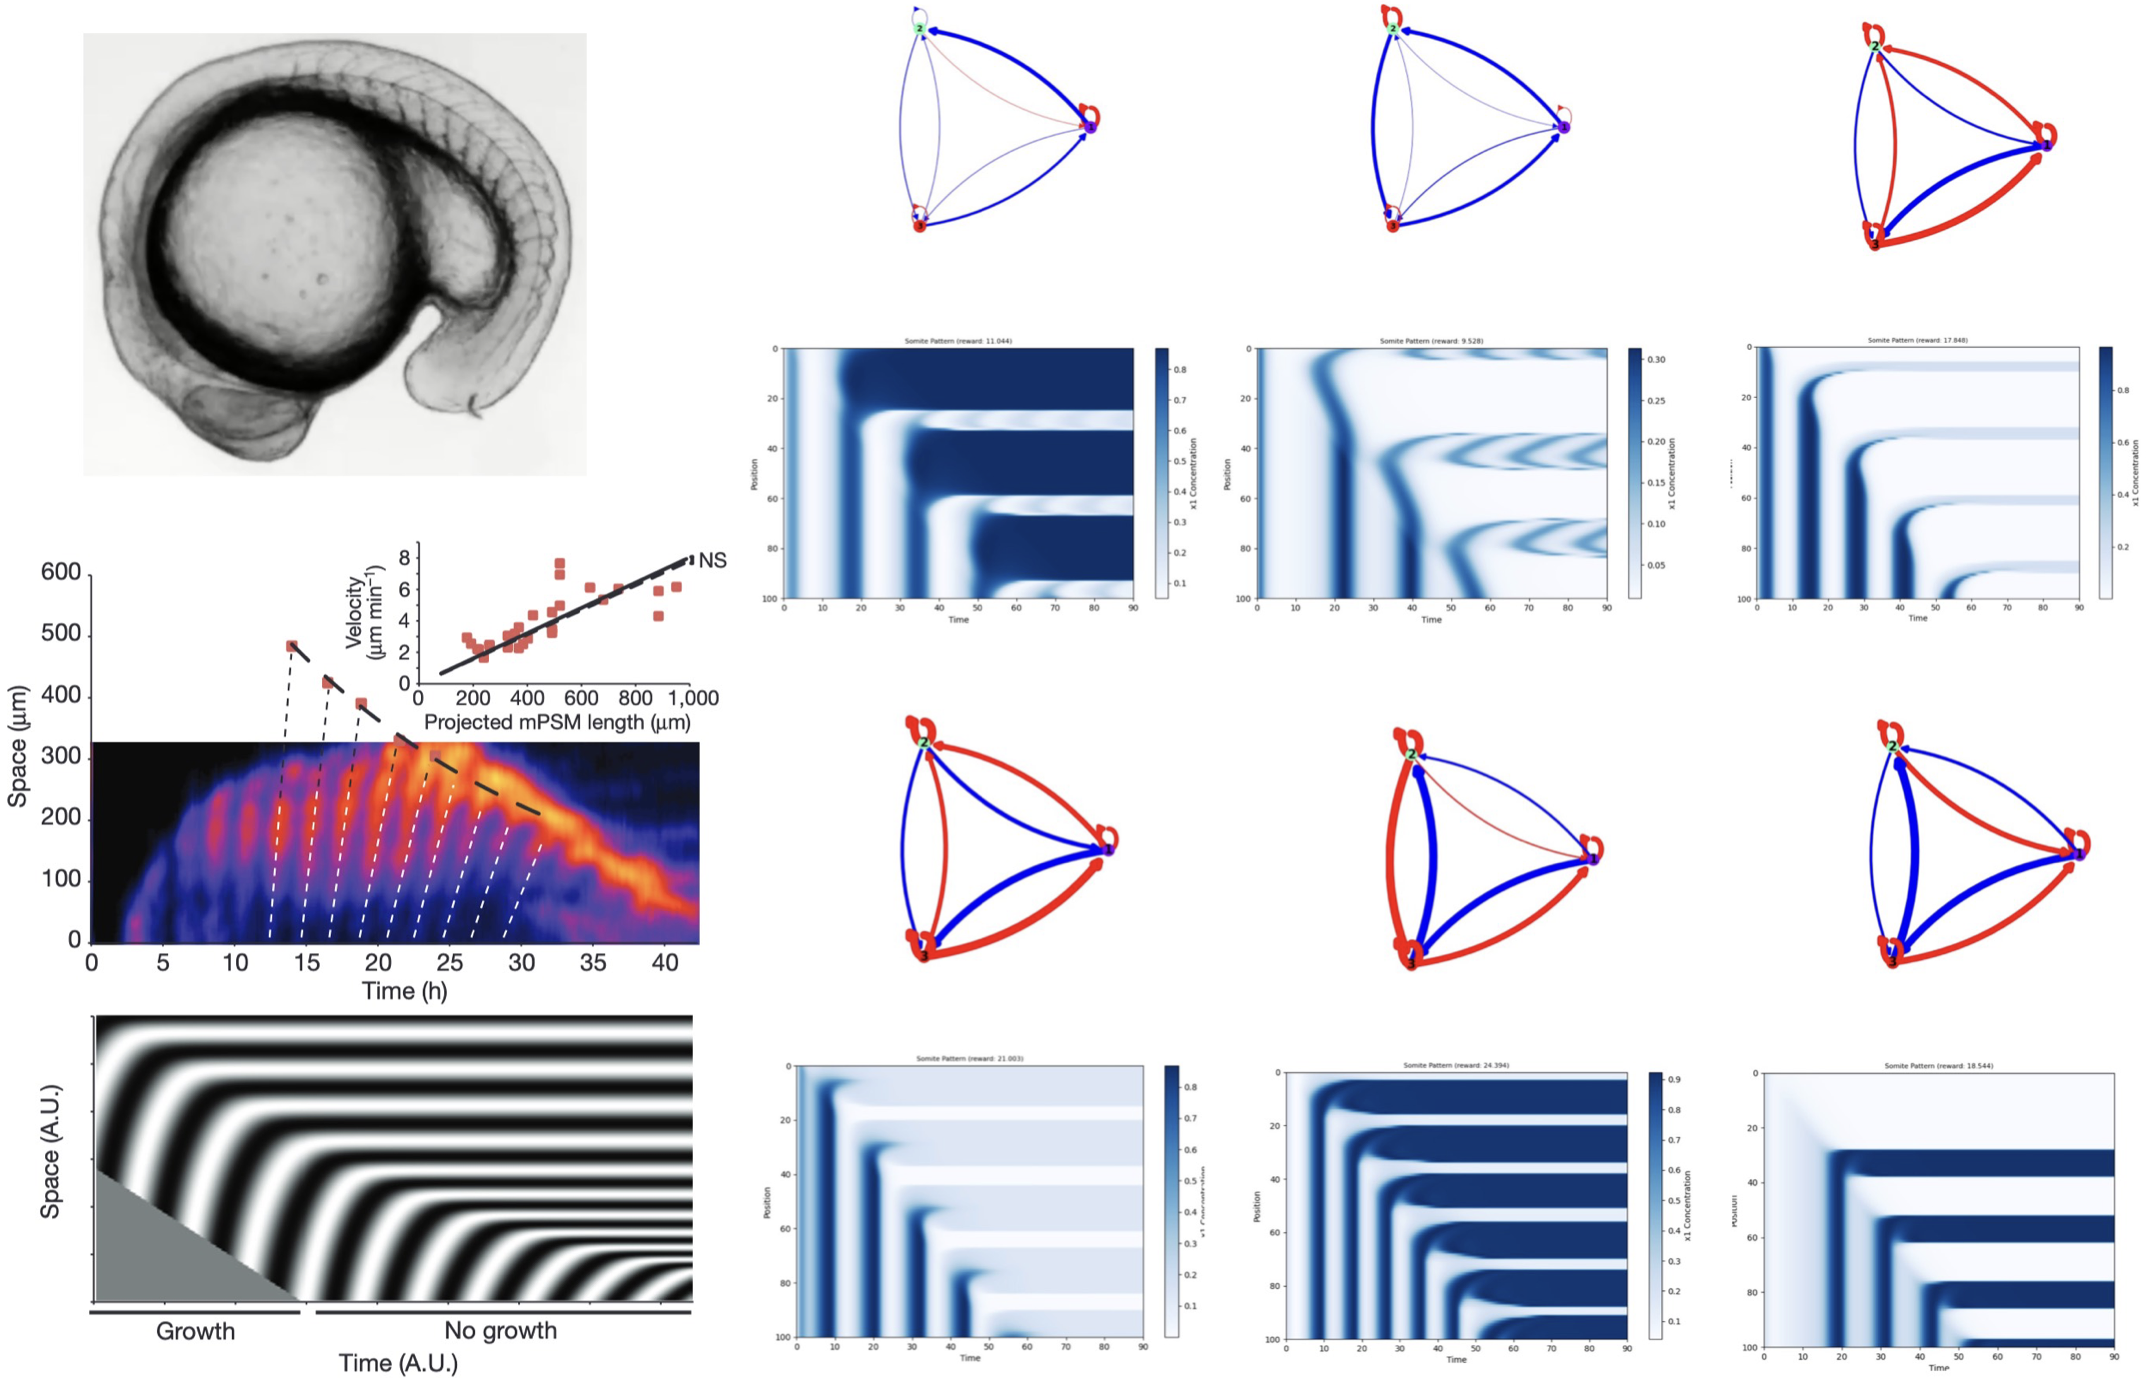
\includegraphics[width = 0.9\textwidth]{./imagesnew/seg.png}
\captionof{figure}{
{\fontfamily{lmss}\selectfont
GFN discovers different network motifs producing diverse segmentation patterns. Experimental images from Lauschke et al., Nature (2013). 
}
}
\end{center}

\vspace{-1.5em}
\begin{center}
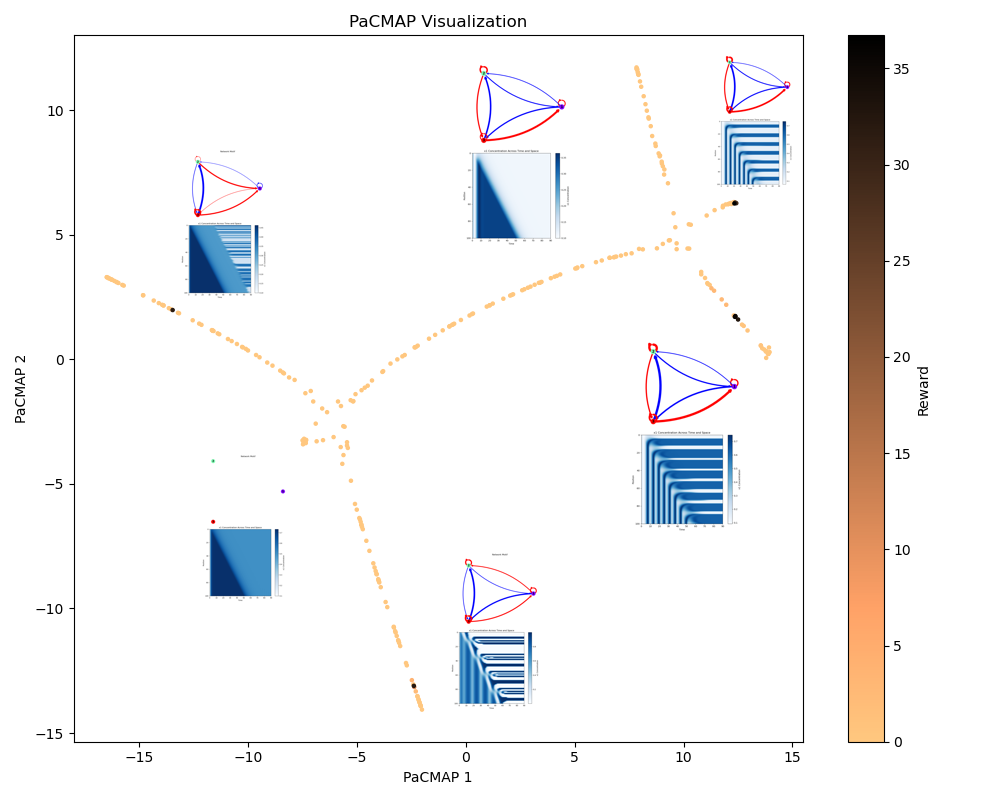
\includegraphics[width = 0.9\textwidth]{./imagesnew/seg_pathway.png} 
\captionof{figure}{
{\fontfamily{lmss}\selectfont
Dim reduction visualization revealing the evolutionary pathways that lead to successful patterning networks. Only top 5 trajectories are shown. 
}
}
\end{center}

}

%%%%%%%%%%%%%%%%%%%%%%%%%%%%%%%%%%%%%%%%%%%%%%%%%%%%%%%%%%%%%%%%%%%%%%%%%%
\headerbox{Key Findings}{name=conclusion,column=2, below=performance}{
%%%%%%%%%%%%%%%%%%%%%%%%%%%%%%%%%%%%%%%%%%%%%%%%%%%%%%%%%%%%%%%%%%%%%%%%%%

% {\bf{\textsf{Key Findings}}}
\vspace{-0.1em}
{\fontfamily{lmss}\selectfont
\begin{flushitem}
    \item Identified diverse motifs achieving specific oscillations in 3-node. 
    \item Discovered common core motifs crucial for dev patterning.
    \item Visualized network evolution trajectories using PaCMAP. 
\end{flushitem}
}

% {\bf{\textsf{Improvements}}}\\
% \vspace{-0.9em}
% \begin{center}
% 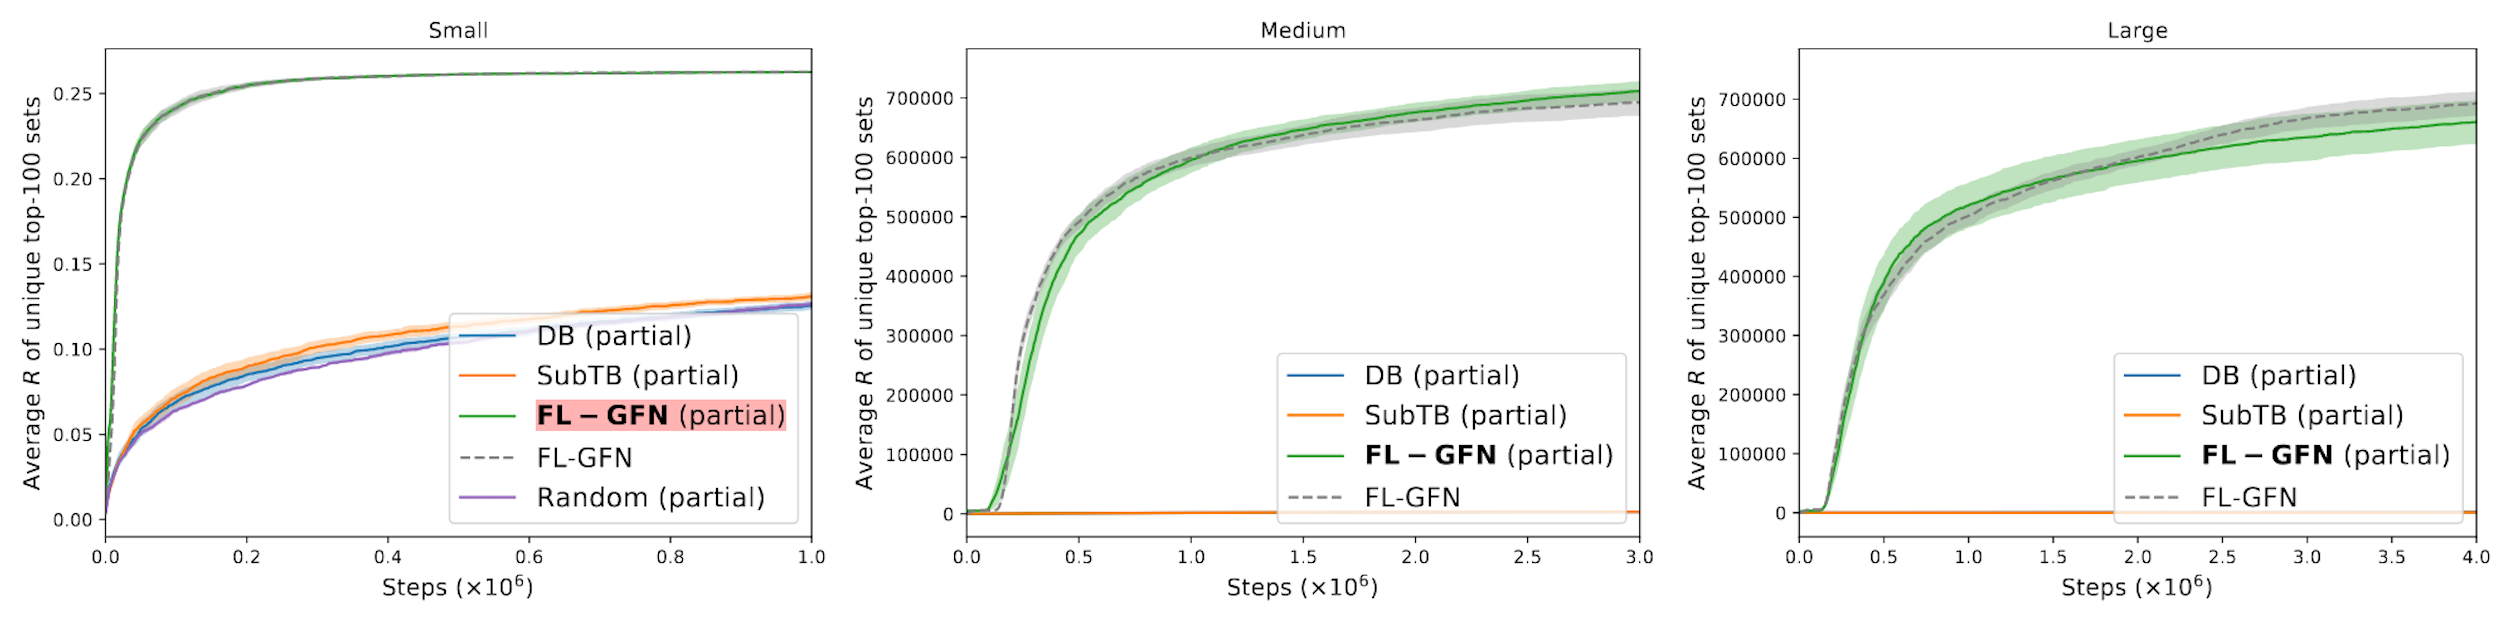
\includegraphics[width = 0.9\textwidth]{./imagesnew/better-training.png}
% \captionof{figure}{
% {\fontfamily{lmss}\selectfont
% Our biological problem involves long trajectories, which poses challenges for GFN training. Several methods including (Ikram et al., 2024; Pan et al., 2024), can be employed to improve GFN performance when dealing with long trajectories and sparse rewards. The figure above is reused from (Pan et al., 2024). 
% }
% }
% \end{center}

}

%%%%%%%%%%%%%%%%%%%%%%%%%%%%%%%%%%%%%%%%%%%%%%%%%%%%%%%%%%%%%%%%%%%%%%%%%%%%%%
%%%%%%%%%%%%%%%%%%%%%%%%%%%%%%%%%%%%%%%%%%%%%%%%%%%%%%%%%%%%%%%%%%%%%%%%%%%%%%%

\end{poster}
\end{document}



% good work!

